\chapter{Introduction}
\label{ch1}

%%%%% https://cerncourier.com/a/pushing-the-precision-frontier/
% https://home.cern/news/news/physics/why-precision-luminosity-measurements-matter

Particle physics studies the fundamental constituents of the Universe, the elementary particles, and the interactions between them, the forces.  To produce and study most of the elementary particles, experiments are carried out in  particle colliders of high energy, where a wide range of technologies are employed to detect and measure the properties of the particles produced, and to measure the collider parameters for its perfomance.\\  This chapter gives a brief background of the elementary particles and particle colliders, as well as relevant concepts-definitions about the measurements studied in this thesis project.

\section{Fundamental Particles}

In our current understanding matter is made up of a group of particles with spin $1/2$, the fermions. The interactions between them, the forces, are described by the exchange of particles, which consist of a group of particles with integer spin: the gauge bosons.
Three of the four forces: electromagnetic force, weak force and strong nuclear force, are mediated by the gauge bosons: photon, $W^{\pm}$ and $Z^{0}$, and gluons ($g$, eight of them), respectively. The description of the gravitational force in particle physics is yet an unresolved challenge. Apart from these vector bosons, there is a special scalar boson called Higgs boson, associated with the mechanism that give mass to all fundamental particles.\\
The group of fermions is categorized in two types: leptons and quarks, giving a total of twelve fundamental particles that compose the matter. There are six leptons, three charged: electron ($e$), muon ($\mu$) and tau ($\tau$), and their corresponding  neutrinos: electron-neutrino ($\nu_{e}$), muon-neutrino ($\nu_{\mu}$) and tau-neutrino ($\nu_{\tau}$). The other group of fermions are the quarks, which cannot be found as individual particles, they can only be found coupled forming particles called hadrons. The group of quarks is formed by the up quark ($u$), down quark ($d$), charm quark ($c$), strange quark ($s$), top quark ($t$) and bottom quark ($q$) \cite{griff}. The force experienced by the fermions is shown in table \ref{tab:table1}.  
\begin{table}[h!]
  \begin{center}
    \caption{Force experienced by the fermions}
    \label{tab:table1}
    \begin{tabular}{l c c c c}
    &    &  \textbf{Electromagnetic} & \textbf{Weak} & \textbf{Strong}\\
      \midrule[1.1pt]
      \multirow{2}{*}{Leptons} & $e$ \hspace{0.3cm}  $\mu$\hspace{0.3cm} $\tau$ & \checkmark & \checkmark & \\ % <-- Combining 2 rows with arbitrary with (*) and content 12
      & $ \nu_{e} $ \hspace{0.3cm}  $\nu_{\mu}$ \hspace{0.3cm} $\nu_{\tau}$  &  & \checkmark\\ % <-- Content of first column omitted.
      \hline
      \multirow{2}{*}{Quarks} & $u$ \hspace{0.5cm}  $c$\hspace{0.5cm} $t$ & \checkmark & \checkmark& \checkmark\\
      & $d$ \hspace{0.5cm}  $s$\hspace{0.5cm} $b$ & \checkmark & \checkmark & \checkmark\\
%      \hline
%      3&3 & 23.113231 & c\\
%      4&4 & 25.113231 & d\\
    \end{tabular}
  \end{center}
\end{table}


All these particles are described by the Standard Model (SM), so far the best theoretical model that provides a successful description of the experimental data.
Most of the experimental data comes from particle colliders because most of the particles of the SM can only be produced and studied using collisions of high energy. One example of this, is the last member of the SM: the Higgs boson, observed in the Large Hadron Collider in proton-proton collisions at energy of $7$ and $8$ $TeV$ in the CMS and ATLAS detectors \cite{higgs_CMS,higgs_ATLAS}.




%%%%%%%%%%%%%%%%%%%%%%%%%%%%%%%%%%%%%%%%%%%%%%%%%%%%%%%%%%%%%%%%%%%%%%%%%%%%%%%%%

\section{Particle Colliders}

Particle physics experiments are designed to detect and identify the particles produced in high-energy collision. The colliding beams produce particle bunch interactions referred to as events. \\
Only the stable and relatively long-lived particles are the observables of particle physics collider experiments. The techniques employed to detect and identify the different particles depends on the nature of their interactions with matter. There are three main types of interactions (broadly speaking): interactions of charged particles, electromagnetic interactions of electrons and photons, and strong interactions of charged and neutral hadrons. The large particle physics detector systems use a wide range of technologies to detect and measure the properties of the particles produced in these high-energy collisions, with the aim of reconstructing the primary particles produced in the interaction from the signals in the different detector systems \cite{thomson_2013}.\\
Apart from the technologies of detection, the most importar features for the performance of a particle collider are its center-of-mass (CM) energy and the luminosity. Achieving a high energy is required to collide %the initial
particles and produce (possibly many) different particles. Some of them with considerably higher masses than the incident particles, for example massive particles such as the $W^{\pm}$, $Z$ and $H$ bosons. The total energy of a incoming particle plus the target particle depends on the reference frame. The frame that is relevant for the production of high mass particles is the CM frame for which the incoming and target particle have equal and opposite momentum of magnitude $p$. Considering the Lorentz invariant quantity $s$ :
\begin{equation*}
s= (E_{1} +E_{2} )^{2}- (\mathbf{p}_{1}+ \mathbf{p}_{2})^{2}c^{2}
\end{equation*}

In the CM frame, where the momenta are equal and opposite, the second term vanishes so that

\begin{equation*}
s= 4 E^{2}
\end{equation*}

where $E$ is the energy of each incoming particle and $s$ is the square of the total incoming energy in the CM frame ;this is a quantity that appears often in particle physics and the notation $\sqrt{s}$ is always used to refer the CM energy. Using  colliding beams of particle with equal mass having the same energy and therefore equal but opposite momentum, makes the experiment taking place in the CM frame and the full energy delivered by the accelerator, $\sqrt{s}=2E$, can be used to produce high mass particles \cite{undergraduate_accelerators_chapter}. Colliding beam machines are used in particle physics experiments due the advantage of  achieving much higher centre-of-mass energies in contrast with a fixed target experiment.\\
The other important parameter of a colllider, the luminosity $\mathcal{L}$, is the quantity that defines ability to produce large numbers of events \cite{ref_lib_vol3}. It quantifies the potential of the collider for delivering a statistically significant sample of a given class of events. A high luminosity is of utmost importance in the search for rare events and new phenomena \cite{lumi_paper_def_and_concept}. This quantity relates the event rates (number of events in time) and the cross section ($\sigma_{p}$) of a particular event; the cross section is a measure of quantum mechanical probability for the interaction. 



\section{Cross section}
In order to illustrate the concept of cross section, we shall consider a simple case where a beam of particles of type $a$, with flux $\phi_{a}$, is crossing a region of space in which there are $n_{b}$ particles per unit volume of type $b$. The interaction rate per target particle $r_{b}$ will be proportional to the incident particle flux, and can be written as \cite{thomson_2013}:

\begin{equation*}
  r_{b}=\sigma \phi_{a}
\end{equation*}

The fundamental physics is contained in $\sigma$, which has dimensions of area, and is termed as interaction cross section. There are cases where the cross section is closely related to the physical cross sectional area of the target, for example, neutron absorption by a nucleus. However, in general, the cross section is simply an expression of the underlying quantum mechanical probability that an interaction will occur \cite{thomson_2013}.\\
Fig. \ref{cs_draw_1} (left) illustrates the definition of cross section, where a single incident particle of type $a$ is travelling with a velocity $v_{a}$ in a region defined by the area $A$, containing $n_{b}$ particles of type$ b$ per unit volume moving with a velocity $v_{b}$ in the opposite direction to $v_{a}$.

\begin{center}
  \begin{figure}[h!]
    \centering
    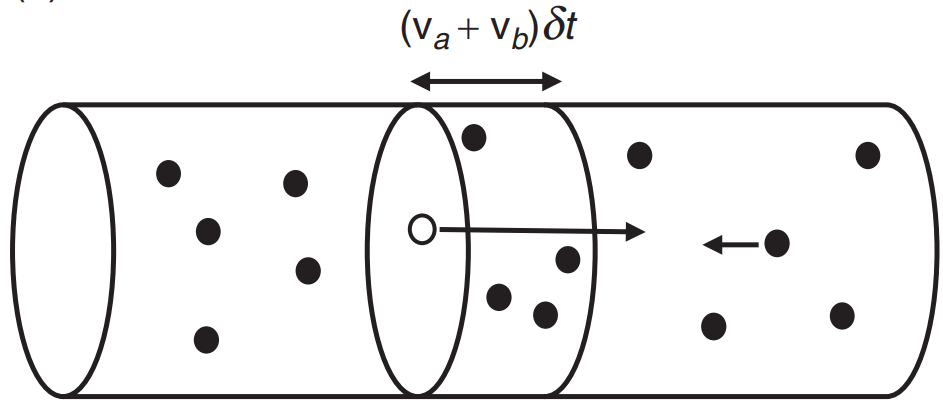
\includegraphics[scale=.25]{Chapter1/cs_draw_1.png} 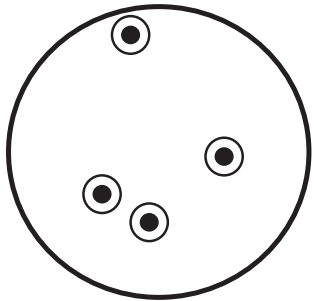
\includegraphics[scale=.25]{Chapter1/cs_draw_2.png}
    \caption[Cross section illustration]{Left: single incident particle of type $a$ traversing a region containing particles of type $b$. Right: projected view of the region traversed by the incident particle in time $\delta t$ \cite{thomson_2013}.}
    \label{cs_draw_1}
  \end{figure}
\end{center}

For a time $\delta t$, the particle a crosses a region containing $\delta N= nb(v_{a}+v_{b}) A \delta t$ of type $b$. The interaction probability can be obtained from the effective total cross sectional area of the $\delta N$ particles divided by the area $A$, which can be interpreted of as the probability that the incident particle passes through one of the regions of area $\sigma$ drawn around each of the $\delta N$ target particles, as shown in Fig. \ref{cs_draw_1} (right) \cite{thomson_2013}. The interaction probability $\delta P$ is therefore

\begin{equation}
\delta P= \frac{\delta N \sigma}{A}= n_{b}v\sigma \delta t
\end{equation}

where $v=v_{a}+v_{b}$. The interaction rate for each particle of type $a$ is

\begin{equation}
r_{a}= \frac{dP}{dt}= n_{b} v\sigma
\end{equation}

For a beam of particles of type $a$ with number density $n_{a}$ confined to a volume $V$, the total interaction rate is

\begin{equation*}
\text{rate}=r_{a}n_{a}V=(n_{b}v\sigma) n_{a}V= (n_{a}v)(n_{b}V)\sigma
\end{equation*}

\begin{equation*}
\text{rate}=\phi N_{b} \sigma
\end{equation*}

so that the total rate is equal to

\begin{equation}
\text{rate}= \text{flux} \times \text{number of target particles} \times \text{cross section}
\end{equation}

Thus, the cross section for a process is defined as

\begin{equation}
\sigma=\frac{\text{number of interaction per unit time per target particle}}{\text{incident flux}}
\end{equation}

where the flux $\phi$ accounts for the relative motion of particles.
%One approach, the simplest one is: 
One approach to calculate the cross section for a particular process can be using the relativistic formulation of Fermi’s golden rule and the appropriate Lorentz-invariant expression for the particle flux.

The cross section for the production of a general final state $O$ at the LHC is given by \cite{lumi_motiv}:
\begin{equation}
  \sigma (pp\rightarrow O +X)= \int dx_{1} dx_{2} \sum_{i,j} f_{i} (x_{1},Q) f_{j}(x_{2},Q) \hat{\sigma}(ij \rightarrow O)(M_{O},g_{ijO}, \cdots)
 \label{cs_theo}
\end{equation}
where $f_{i}(x,Q)$ is the density fo partons\footnote{Before quarks and gluons were generally accepted, Feynman proposed that the proton was made up of point-like constituents, termed partons \cite{thomson_2013}.} (PDF) of type $i$ (quarks of different flavours or gluons) inside the proton, carrying a fraction $x$ of the proton momentum at a resolution scale $Q$. Theory predicts the PDFs to be independent of $O$. $\hat{\sigma}(ij \rightarrow O)$ is the partonic cross section to produce the final state $O$ in the collisions of partons $i$ and $j$. It depends on properties of the final state (for example the mass of $O$, $M_{O}$, the momentum of the various particles involved, etc.), and on the the nature of the interactions involved in the process (for example the strength, $g_{ijO}$, of the coupling between $i$, $j$ and $O$). Parameters like $M_{O}$ and $g_{ijO}$ are therefore what defines the underlying theory, and extracting their value as accurately as possible is the ultimate goal of an experimental measurement \cite{lumi_motiv}.
The precision of the extraction of these parameters is determined by \cite{lumi_motiv}:
i) The precision of the calculation of $\hat{\sigma}(ij \rightarrow O)$ as a function of $M_{O}$, $g_{ijO}$, etc.; this is a theoretical aspect. Inclusion of higher and higher orders of perturbation theory makes the prediction more accurate.
ii) The precision of the knowledge of the PDFs; a theoretical and experimental aspect. For example, experimental data from measurements such as deep inelastic scattering (DIS) are necessary to extract the PDFs, by fitting these data to the DIS equivalent of an equation like \ref{cs_theo}. Likewise, is expected to use the LHC data themselves to improve the knowledge of the PDFs, by including the functions $f_{i}$ to the list of parameters in eq. \ref{cs_theo} that are allowed to float in order to fit the data.


\section{Luminosity }

Luminosity, $\mathcal{L}$ , is defined as the proportionality factor between the number of events per second $R$ (event rates) and the cross section $\sigma_p$ for a given process $p$ \cite{ref_lib_vol3}:

\begin{equation}
R=\mathcal{L}_{inst} \cdot \sigma_{p}
\end{equation}

Cross section has units $cm^{2}$, therefore the unit of luminosity is $cm^{-2}s^{-1}$.\\
To derive a general expression of luminosity, we will consider the case of colliding beams at head-on.
%a relevant case for LHC context[relibvol3]. foot page?
At head on collision, the instantaneous luminosity for $N_{b}$ colliding bunches is given by:

\begin{equation}
  \mathcal{L}_{inst}= N_{b} N_{1}N_{2}f \int_{-\infty}^{\infty} dx\int_{-\infty}^{\infty} dy \rho_{1}(x,y)\rho_{2}(x,y)
    \label{lumi_1}
\end{equation}

where $N_{1,2}$ are the particles per bunch, $f$ the revolution frequency and $\rho_{1,2}$ are the distribution functions of the two beams in the transverse plane. Assuming that $\rho$ can be factorized into independent terms in $x$ and $y$, i.e. uncorrelated bunch densities in all planes:

\begin{eqnarray}
  \rho_{i}(x,y)= \rho_{i}(x)\rho_{i}(y) & &i=1,2
\end{eqnarray}

So that eq. \ref{lumi_1}

\begin{equation}
  \mathcal{L}_{inst}= N_{b} N_{1}N_{2}f \int_{-\infty}^{\infty}\rho_{1}(x)\rho_{2}(x)  dx\int_{-\infty}^{\infty}\rho_{1}(y)\rho_{2}(y) dy
    \label{lumi_2}
\end{equation}

If the bunch densities have Gaussian profile in both directions, i.e 

\begin{eqnarray}
\rho(u)= \frac{1}{\sqrt{2\pi} \sigma_{u}} exp \biggl(-\frac{u^{2}}{2\sigma_{u}^{2}} \biggr)&  &  u=x,y
\end{eqnarray}

The integration yields
\begin{equation}
  \mathcal{L}_{inst}= \frac{N_{1} N_{2} N_{b}f }{4\pi \sigma_{x} \sigma_{y}}
  \label{lumi_theor}
\end{equation}

In practice, the properties of the colliding beams are not know precisely, such as the bunch density profile, so that the integral in  \ref{lumi_2} cannot be solved analytically. In LHC a experimental technique is implemented with a dedicated machine setup to estimate the integrals, yielding a similar expression as \ref{lumi_theor}. This is discussed in chapter \ref{ch3}.\\
%%%%%%%%%%%%%%%%%%%%%%NEW%%%%%%%%%%%%%%%%%%%%%%%%%%%%%%%%%%%%%%%
%Luminosity  is a general concept that can be interpreted from geometry and flux of particles per unit of time. Considering two bunches of particles $N_{1,2}$ in a circular collider, colliding in an interaction region as shown in Figure 2.1. , the luminosity is expressed as [Simón-these]:
%\begin{equation}
%\mathcal{L}= \frac{N_{1}N_{2}f}{A_{eff}}
%\end{equation}
%where $A_{eff}$ is the effective transverse area in which the collisions take place and $f$ is the revolution frequency. The only unknown parameter that needs to be measured is the effective transverse area. 
%%%%%%%%%%%%%%%%%%%%%%%%%%%%%%%%%%%%%%%%%%%%%%%%%%%%%%%%%%%%%%%
The instantaneous luminosity measure is of great importance beacuse it reflects the performance of the collider, but  this is not the only measurement concerned with luminosity. Another important measurement of luminosity is the integrated luminosity \cite{ref_lib_vol3}:

\begin{equation}
  \mathcal{L}_{int}=\int_{0}^{T} \mathcal {L}_{\text{inst}}(t) dt
\end{equation}

The integral is taken over a period of time $T$ (excluding possible dead time). The integrated luminosity has units of $cm^{-2}$ and is often expressed in inverse barn ($1 barn= 10^{-24}cm^{2}$). The importance of the integrated luminosity  is because it directly relates to the number of observed events: $ \mathcal{L}_{int}\cdot \sigma_{p}$. \\Another important parameter for a beam with high luminosity and bunched beams are the number of particle collisions per bunch crossing, called pileup ($\mu$). Pileup and luminosity are related by  $f \mu= \mathcal{L}_{\text{inst}} \sigma_{p}$ .\\
Up to date, the particle collider with the highest luminosity and energy is the Large Hadron Collider (LHC) built by CERN, located in 	Geneva, Switzerland.


%\subsection{Luminosity measurement}

%Experimentally, the luminosity is measured with luminometers, which reads out a rate of the specific quantities observed in the detector (hits, tracks, clusters, etc.). This rate, R, should be proportional to the instantaneous luminosity , $\mathcal{L}_{inst}$, with the constant of proportionality given by the visisble cros section $\sigma_{vis}$ [pas-18 ?]:

%\begin{equation}
%R= \mathcal{L}_{inst} \sigma_{vis}
%\end{equation}

%The determination of $\sigma_{vis}$ is carried out throuhg vand der Meer (vdM) scans performed with a dedicated LHC machine setup. In the practice, the assumption [simon tese cern thesis] of the gaussian profile can not be known, and the integrals are solved using the van der Meer method, yielding a similar expression for Luminosity as the previous one. So that lumi expresion is substituted in eq prev and sigma vis obtained.

\section{Importance of Luminosity precision}

The precision of the measured cross section, $\sigma_{exp}(O)$, is determined by the quantities on the right hand-side of: $\sigma_{exp}(O) = N_{\text{events}}(O)/\mathcal{L}_{int}$. $N_{\text{events}}$ depends on the accurate knowledge of signal and background acceptances and efficiencies. \\
The target of the programme of precision measurements is therefore to bring to the same level the accuracy of all elements in the following relation:
$$\sigma (pp \rightarrow O)= \frac{N_{\text{events}}(O)}{\mathcal{L}_{int}}$$
The possibility to have a very accurate absolute luminosity determination, and therefore very accurate experimental cross section measurements, allows to develop a physics programme in which this precise information can help improve, at the same time, the theoretical calculations, the PDF knowledge, and ultimately the measurement of the theory parameters such as masses and couplings\cite{lumi_motiv}. 
The experimental techniques to determine signal rates are mature enough, where the understanding of acceptances, detector biases, reconstruction efficiencies or background subtraction is at the subpercent level, so that the final precision of the physics measurement is dominated by the luminosity uncertainty \cite{lumi_paper_def_and_concept}. \\
The precision in the measurement of the luminosity directly impacts the precision in the measurement of the cross section, and therefore has a large impact in our understanding of the Standard Model parameters.



\section{The Large Hadron Collider}

The LHC was designed to collide proton beams with a centre-of-mass energy of 14  TeV and a luminosity of $10^{34}cm^{-2}s^{-1}$. It was also designed to collide heavy ($Pb$) ions with an energy of 2.8 TeV per nucleon and a peak luminosity of $10^{27}cm^{-2}s^{-1}$ \cite{lhcmachine2008}.\\
The LHC consists of two rings of 27 km of circumference which guide accelerated bunches of protons (or Pb) at high energy to collide. Figure \ref{lhc_com} shows the CERN accelerator complex. The bunches are previously accelerated by a chain of pre-accelerators. First, protons are produced by ionizing hydrogen and then are transferred to the Linear Accelerator 2 (LINAC2) where the protons are accelerated in bunches up to an energy of 50 MeV, and then the bunches pass trough three circular accelerator: the Booster, the Proton Synchrotron (PS) and the Super Proton Synchrotron (SPS), giving an energy of 1.4 GeV, 26GeV and 450 GeV, respecectively. After these three preaccelerators, the bunches are finally circulating in oposite directions in the LHC ring, where are further accelerated to reach energies up to 7 TeV (per bunch). This entire procedure defines a single LHC fill generally consisting of $10^{14}$ protons, grouped into bunches to form the proton beam.\\
There are four experiments placed around the LHC ring: Compact Muon Solenoid (CMS) \cite{CMS_Exp_2008}, A Toroidal LHC ApparatuS (ATLAS) \cite{Atlas_Exp_2008}, A large Ion Colliding Experiment (ALICE) \cite{ALICE_Exp_2008} and LHCb \cite{LHCb_Exp_2008}. CMS and ATLAS are for general-purpose detectors to investigate the largest range of SM and Beyond SM (BSM) physics. ALICE and LHCb have detectors specialized to study specific phenomena.

\begin{center}
  \begin{figure}[ht]
    \centering
    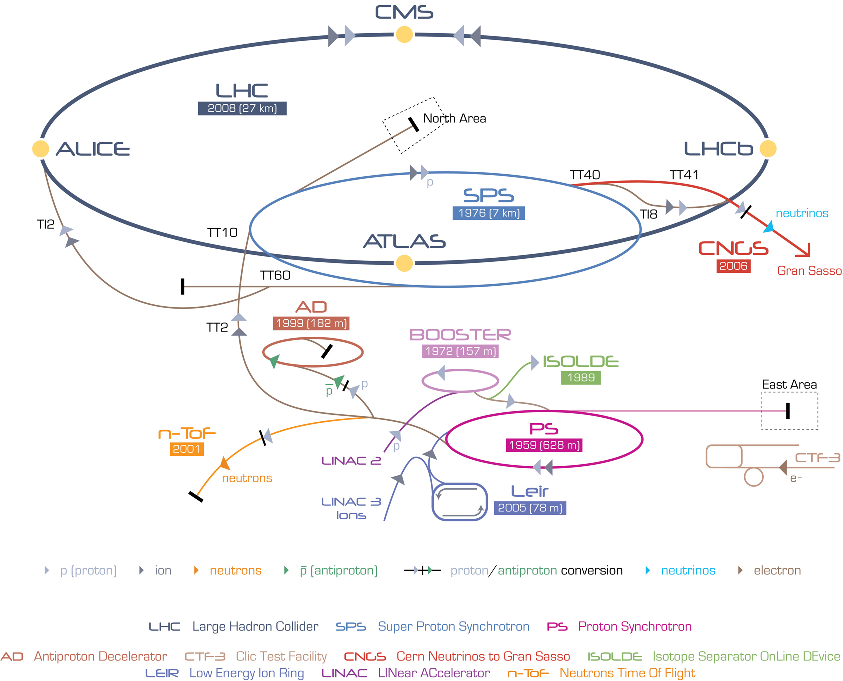
\includegraphics[scale=.41]{Chapter1/lhc_complex_fig.png}
    \caption[LHC Complex]{Diagram of the LCH complex \cite{lhc_complex}.}
    \label{lhc_com}
  \end{figure}
\end{center}




\section{LHC Luminosity}
The LHC has had two Runs and two long shutdowns for maintenance and  upgrades. Run 1 lasted from 2010-2012, while Run 2 lasted from 2015-2018. In Run1, LHC reached a peak instantaneous luminosity of  $0.77 \times 10^{34}$  and an integrated luminosity of $25 fb^{-1}$  for proton-proton collisions at $\sqrt{s}=\text{8 TeV}$ in 2012\cite{LHC_status_2013}. For the first part of Run-2 (2015-2016) in proton-proton colissions at $\sqrt{s}=\text{13TeV}$ in CMS detector, the integrated luminosities when CMS was fully operational are $2.2$7 and $36.3$ $fb^{-1}$ in 2015 and 2016, with a relative precision of 1.6\% and 1.2\%, respectively \cite{lumi_precise_2015_2016}. For the second part of Run 2 (2017-2018), the integrated luminosity is about $49.8 fb^{-1} $ and $67.9 fb^{-1}$ for 2017 and 2018, respectively, as can be seen in Fig. \ref{lumi_per_year_int}. The total systematic uncertainty in the calibration of luminosity measurement is 2.3\% in 2017\cite{pas_17} and 2.5\% in 2018 \cite{pas_18}, but its precision remains to be improved. The main objective of this thesis project is to contribute to the improvement of the precision of 2018 luminosity calibration.


\begin{center}
  \begin{figure}[h!]
    \centering
    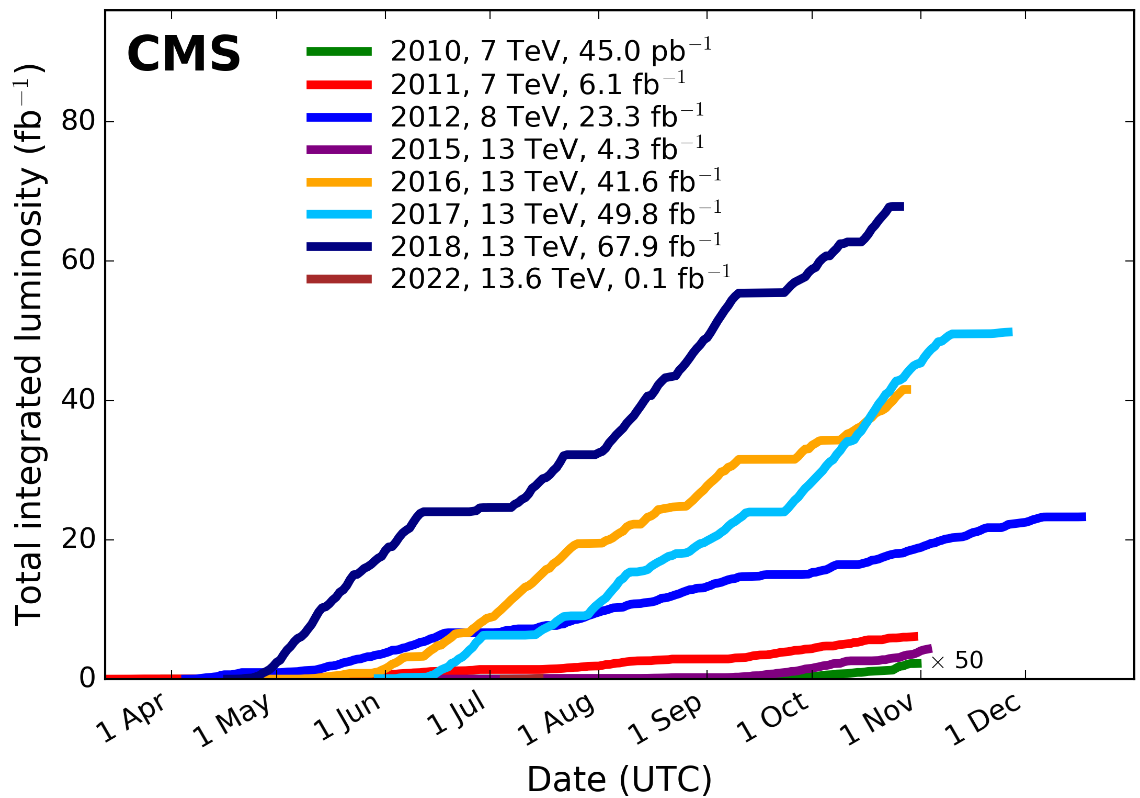
\includegraphics[scale=.3]{Chapter1/int_lumi_per_year.png}
    \caption[CMS Luminosity per year]{Delivered luminosity versus time for Run-1 (2010-2012) and Run-2 (2015-2018); pp data only. Cumulative luminosity versus day delivered to CMS during stable beams for pp collisions at nominal center-of-mass energy. These plots use the best available offline calibrations for each year. For 2017 and  2018 the plots are based on \cite{pas_17} and \cite{pas_18}, respectively \cite{wikicern}.}
    \label{lumi_per_year_int}
  \end{figure}
\end{center}

%lumi values:
% https://inspirehep.net/files/11b4a1d6569e8e066e7431f17a55d69c

% https://arxiv.org/pdf/1504.06519.pdf

%ATLAS 2015-2018: https://arxiv.org/pdf/1911.04632.pdf
